\chapter{Results}

\section{Our Contributions}

In this section we will present and reiterate the contributions we have made as a result of this project.

We have contributed with a simplified Python version of the original GFN2-xTB Fortran implementation. The implementation and validation of the dispersion term is not complete, and we have not implemented the self-consistent charges that is used to iteratively rerun the computations to improve the accuracy of the result. Given the size of the reference implementation we are quite satisfied with this. The Python implementation should hopefully make the GFN2-xTB algorithm more approachable for our successors and give a good foundation for making the lockstep parallel GPU implementation.

We have contributed a testing framework for comparing results against the original Fortran implementation. We utilize Nix to ensure tests that are reproducible, regardless of Linux distribution and system configuration. In connection to this, we have also contributed a reproducible and easy way to build, run, and patch xtb. This also includes its dependencies, and even the older GPU compatible version 6.4.0 of xtb known from GitHub issues to be difficult to run.

This report contributes a walkthrough of the GFN2-xTB algorithm with code snippets that directly links to the equations in a way that should be more easily digestible for a computer scientist. As an extension of this, we have presented insights and ideas on how to approach a massively lockstep implementation by optimizing code snippets for our problem domain, and transforming them such that they adhere to the requirements of a lockstep kernel.

We have also presented a case study with the NVIDIA A100 datacenter GPU to show how GPU architectures are structured and how to use the technical specifications to estimate hardware requirements.


% TODO: ASMUS!!!! Skriv vores quantum contributions >w<
%In continuation of this, we have designed our own quantum circuits and proposed how to use the arithmetic operations they implement to further optimize the xTB algorithm with computational quantum algorithmic approaches.

\section{Validation}

All of our tests pass indicating that our results match the reference implementation. We had to introduce a threshold for some of the comparisons as they came extremely close. \autoref{fig:validation_electro_precision} shows the maximum squared deviations of all tests for the electrostatic term. This term returns the isotropic electrostatic energy and the self-consistent charges, so there are two plots to show both.

\begin{figure}[H]
\centering
\begin{subfigure}{.5\textwidth}
  \centering
  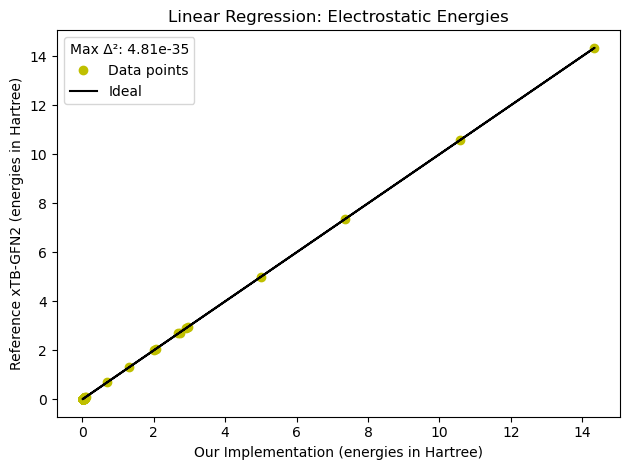
\includegraphics[width=.9\linewidth]{images/results/es_check}
  \label{fig:es_check}
\end{subfigure}%
\begin{subfigure}{.5\textwidth}
  \centering
  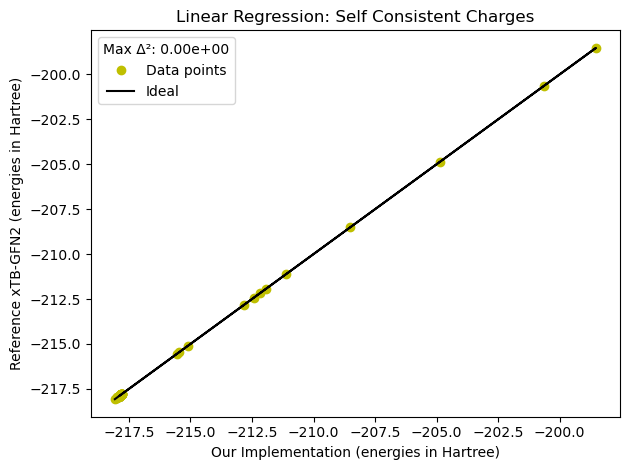
\includegraphics[width=.9\linewidth]{images/results/scc_check}
  \label{fig:scc_check}
\end{subfigure}
\caption{Linear regressions showing how much the Python implementation for the electrostatic term deviates from the Fortran results.}
\label{fig:validation_electro_precision}
\end{figure}

\section{Benchmarks}
